%%
%% Copyright 2007, 2008, 2009 Elsevier Ltd
%%
%% This file is part of the 'Elsarticle Bundle'.
%% ---------------------------------------------
%%
%% It may be distributed under the conditions of the LaTeX Project Public
%% License, either version 1.2 of this license or (at your option) any
%% later version.  The latest version of this license is in
%%    http://www.latex-project.org/lppl.txt
%% and version 1.2 or later is part of all distributions of LaTeX
%% version 1999/12/01 or later.
%%
%% The list of all files belonging to the 'Elsarticle Bundle' is
%% given in the file `manifest.txt'.
%%

%% Template article for Elsevier's document class `elsarticle'
%% with numbered style bibliographic references
%% SP 2008/03/01
%%
%%
%%
%% $Id: elsarticle-template-num.tex 4 2009-10-24 08:22:58Z rishi $
%%
%%
\documentclass[preprint,12pt]{elsarticle}

%% Use the option review to obtain double line spacing
%% \documentclass[preprint,review,12pt]{elsarticle}

%% Use the options 1p,twocolumn; 3p; 3p,twocolumn; 5p; or 5p,twocolumn
%% for a journal layout:
%% \documentclass[final,1p,times]{elsarticle}
%% \documentclass[final,1p,times,twocolumn]{elsarticle}
%% \documentclass[final,3p,times]{elsarticle}
%% \documentclass[final,3p,times,twocolumn]{elsarticle}
%% \documentclass[final,5p,times]{elsarticle}
%% \documentclass[final,5p,times,twocolumn]{elsarticle}

%% if you use PostScript figures in your article
%% use the graphics package for simple commands
%% \usepackage{graphics}
%% or use the graphicx package for more complicated commands
%% \usepackage{graphicx}
%% or use the epsfig package if you prefer to use the old commands
%% \usepackage{epsfig}

%% The amssymb package provides various useful mathematical symbols
\usepackage{amssymb}
\usepackage{xcolor}
%% The amsthm package provides extended theorem environments
%% \usepackage{amsthm}

%% The lineno packages adds line numbers. Start line numbering with
%% \begin{linenumbers}, end it with \end{linenumbers}. Or switch it on
%% for the whole article with \linenumbers after \end{frontmatter}.
%% \usepackage{lineno}

%% natbib.sty is loaded by default. However, natbib options can be
%% provided with \biboptions{...} command. Following options are
%% valid:

%%   round  -  round parentheses are used (default)
%%   square -  square brackets are used   [option]
%%   curly  -  curly braces are used      {option}
%%   angle  -  angle brackets are used    <option>
%%   semicolon  -  multiple citations separated by semi-colon
%%   colon  - same as semicolon, an earlier confusion
%%   comma  -  separated by comma
%%   numbers-  selects numerical citations
%%   super  -  numerical citations as superscripts
%%   sort   -  sorts multiple citations according to order in ref. list
%%   sort&compress   -  like sort, but also compresses numerical citations
%%   compress - compresses without sorting
%%
%% \biboptions{comma,round}

% \biboptions{}


\journal{Nuclear Physics B}
\graphicspath{{images/}}

\begin{document}

\begin{frontmatter}

%% Title, authors and addresses

%% use the tnoteref command within \title for footnotes;
%% use the tnotetext command for the associated footnote;
%% use the fnref command within \author or \address for footnotes;
%% use the fntext command for the associated footnote;
%% use the corref command within \author for corresponding author footnotes;
%% use the cortext command for the associated footnote;
%% use the ead command for the email address,
%% and the form \ead[url] for the home page:
%%
%% \title{Title\tnoteref{label1}}
%% \tnotetext[label1]{}
%% \author{Name\corref{cor1}\fnref{label2}}
%% \ead{email address}
%% \ead[url]{home page}
%% \fntext[label2]{}
%% \cortext[cor1]{}
%% \address{Address\fnref{label3}}
%% \fntext[label3]{}

\title{}

%% use optional labels to link authors explicitly to addresses:
%% \author[label1,label2]{<author name>}
%% \address[label1]{<address>}
%% \address[label2]{<address>}

\author{}

\address{}

\begin{abstract}
%% Text of abstract
Recently machine learning methods had gain lots of publicity among researchers in order to analyze the brain images such as functional Magnetic Resonance Imaging(fMRI) to obtain a better understanding of the brain and its related disease such as Alzheimer's disease. Different methods have been deployed in order to discriminate Alzheimer's disease from normal ones which is a hard task, especially in early stages (eMCI) case. The majority of deployed techniques rely on constructing the functional connectivity (FC) for each person and use the vectorized FC as the input for the classifiers which has two main drawbacks: 1) The need for constructing the FC 2) The loss of possible valuable structural information in the vectorization step.
    Considering these problems and based on multidimensional nature the data, we have came up with a novel framework which omits the FC construction part and preserve the structural integrity of data for the classification.
        The proposed framework uses the High Order Singular Value Decomposition (HOSVD) in order to prune the classes and select the proper basis for each of them.
This framework also allows us to obtain a general FC pattern for normal and eMCI classes but not a single sample which helps us to shed more lights on the brain abnormalities in the Alzheimers disease at its early stages. 
        Extensive experiments using the ADNI dataset demonstrate that
        our proposed framework effectively boosts the fMRI classification performance and reveals novel connectivity patterns in Alzheimer's disease at its early stages.
\end{abstract}

\begin{keyword}
%% keywords here, in the form: keyword \sep keyword

%% MSC codes here, in the form: \MSC code \sep code
%% or \MSC[2008] code \sep code (2000 is the default)

\end{keyword}

\end{frontmatter}

%%
%% Start line numbering here if you want
%%
% \linenumbers

%% main text
\section{Introduction}
\label{Intro}
Alzheimer’s disease (AD) is a progressive neurodegenerative disorder with a long pre-morbid asymptomatic period which affects millions of elderly individuals worldwide\cite{r01}. It is predicted that the number of affected people will double in the next 20 years, and 1 in 85 people will be affected by 2050 \cite{r02}. The predominant clinical symptoms of AD include a decline in some important brain cognitive and intellectual abilities, such as memory, thinking, and reasoning. Precise diagnosis of AD, especially at its early warning stage: early Mild Cognitive Impairment (eMCI), enables treatments to delay or even avoid such disorders \cite{r03}.

In recent years, brain imaging techniques like Positron Emission Tomography(PET)\cite{r21}, Electroencephalography (EEG)\cite{r22}
	 and functional Magnetic Resonance Imaging (fMRI)\cite{r23} 
	 have been used in analysis of AD. Due to the high spatial resolution and relatively lower costs, fMRI is vastly used among researchers in order to monitor brain activities especially in AD and all its stages in which detecting abnormalities within small brain regions is essential \cite{r04}. 
	An fMRI sample is naturally a 4D tensor consisting of 3D voxels moving in time, and each voxel contains an intensity value that is proportional to the strength of the Blood Oxygenation Level Dependent(BOLD) signal, which is a measure of the changes in blood flow, to estimate the activity of different brain regions\cite{r07}.
	Resting-state fMRI(rs-fMRI) is an fMRI technique in which the patient is asked to rest during the whole scan, focuses on the low-frequency $\left( < 0.1 Hz \right)$  oscillations of BOLD signal, which presents the underlying neuronal activation patterns of brain regions[8]–[10]. rs-fMRI is usually used in order to analyze brain diseases like AD or autism\cite{r33,r34}.
	%
	%Since the number of voxels within a single full scan is high 
	%($5000$ up to roughly $200,000$[ref(Definingnodes)]) and they form strong spatial relations, 
	
	Since each fMRI volume consist of hundreds of thousands of voxels which are often highly correlated with the surrounding voxels in the brain volume, parcellation of the brain for further analysis has moved toward the use
	of anatomical atlases. These atlases are strictly defined using
	anatomical features of the brain, like locations of common gyri
	and do not rely on any functional information.
	To generate data
	using an Atlas based approach, the BOLD signal from all voxels is averaged within each brain region called Region of Interest(ROI)\cite{r09}.
	By putting together the average time-series for all the ROIs, the $i$th volume would become $X_i \in \mathbb{R}^{T \times R} , i = \{1,2,\cdots, S\}$ in which $R$, $T$ and $S$ are the number of ROIs, time points and samples respectively. 
	The process of obtaining such a matrix is shown in Figure \ref{g1.1}.% 
			\begin{figure*}[!t]
			\centering
			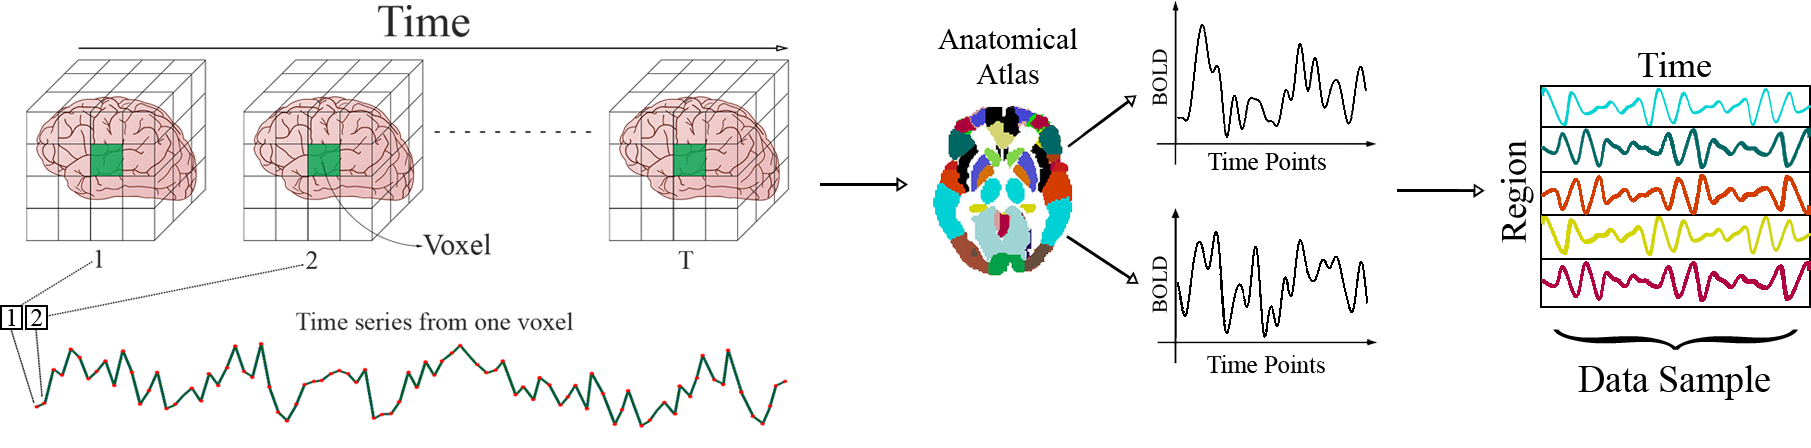
\includegraphics[width=5.5in]{Data}
			\caption{The process of extracting ROI time-series from the original 4D volume. }
			\label{g1.1}
		\end{figure*}
	
	  There are two major studies associated with rs-fMRI data: finding common brain disorders caused by diseases like Alzheimer's or autism, and more recently detecting patients with brain disorders using classification techniques \cite{r35,r36}. Due to the high dimensionality of data and the nature of diseases like eMCI which does not show any reliable clinical symptoms,
	    researchers moved towards advanced machine learning techniques in order to achieve more reliable analysis \cite{r37}.
	    
	    	There are two major studies associated with rs-fMRI data: finding common brain disorders caused by diseases like Alzheimer's or autism, and more recently detecting patients with brain disorders using classification techniques \cite{r35,r36}. Due to the high dimensionality of data and the nature of diseases like eMCI which does not show any reliable clinical symptoms,
	    	researchers moved towards advanced machine learning techniques in order to achieve more reliable analysis \cite{r37}.
	    	
	A powerful tool that is commonly used in order to achieve aforementioned goals is Functional Connectivity(FC) network.  FC is a $region \times region$ matrix $\bar{X}$ in which $\bar{x}_{ij}$ represents the functional connectivity between the $i$th and $j$th ROI. Functional connectivity is an observable
		phenomenon quantifiable with measures of statistical dependencies, such as correlations, coherence, or transfer entropy \cite{r38}.  Recent studies have shown that some brain disorders like AD could alter the way that some brain regions interact with each other. For example, compared with the healthy, AD patients have been found decreased functional connectivity between the hippocampus and other brain regions, and MCI patients have been observed increased functional connectivity between the frontal lobe and other brain regions??.
		\textcolor{red}
		{So, Finding an FC that highlights the patterns caused by a disease has been a common goal in the rs-fMRI study for a long time. Several approaches exist to find common patterns among different brain scans. Data-driven methods such as kernel-PCA or clustering techniques have been proposed for this task\textcolor{red}{ref?}. But ultimately most of them rely on calculating a network for each volume. This may overlook the role of noises or outliers within the data. }
	
		In recent years FCs are also used as features in classification. 
				So, instead of using $X_i$ as the $i^{th}$ sample its corresponding  FC i.e. $\bar{X}_i$ is used as a feature. Although FCs show promising results, they bring their own challenges.  The computational cost of FC usually is high and also its quality has a main effect in the quality of learning process. Also, Since the conventional classifiers like SVM work on data in vector format, these matrix features should be vectorized in order to feed them to classifiers.
				This vectorization leads to high-dimensional vectors which produce poor performance due to the phenomena known as the Curse of Dimensionality.Alongside the curse of dimensionality, vectorization also destroys potential information that are embedded in the structure of data. 
						This problem has been studied especially in image data in which vectorization destroys the spatial relations within an image.\textcolor{red}{Rezghi and S.Ahmadi paper}
						
						
	In this paper, based on high order tensor decomposition, we have created a framework in which the mentioned goals i.e. finding an FC for a whole class and detecting a disorder via classification could be achieved via a single High Order Singular Value Decomposition (HOSVD) of each class.
	 Here based on latent variables obtained by HOSVD a general representative pattern of FC for eMCI and normal are obtained. Experiments show that the functional connectivities by the proposed method are confirmed by empirical methods along with novel connectivities. Also, The proposed classifier also outperforms state of the art eMCI classification methods. 
	 Viewing each class as a tensor allows us to work with \textit{time} and \textit{region} features separately but simultaneously. This multilinear view
	  ables us to design a proper dimension reduction relative to the nature of each feature along with a discriminant function based on linear regression \textcolor{red}{on latent space of samples} that uses the test data to enhance the quality of the training set without forcing any a prior knowledge to the classifier, a task which is not possible through well known classifiers like SVM, logistic regression or k-NN. It is also notable that the proposed discriminant function directly works with the $X_i$s as features. Having the FC calculation step omitted not only heavily affects the computational performance of the method, but it also saves us from the troubles of FCs mentioned before.   
	  
	  To verify our approach, we conduct an extensive experimental study on rs-fMRI data from the
	  	benchmark dataset ADNI
	  	\footnote{http://adni.loni.usc.edu/} 
	  	As will be seen, the results well demonstrate the effectiveness and advantages of our method. Specifically, the proposed framework, not only grants us superior classification accuracy to that from other methods, it is also much faster and more stable against different data selection schemes. We have also confirmed our achieved whole-class FC matrix using empirical data on the eMCI and Normal functional connectivity patterns.
	  	
							 
				
				
\section{}

%% The Appendices part is started with the command \appendix;
%% appendix sections are then done as normal sections
%% \appendix

%% \section{}
%% \label{}

%% References
%%
%% Following citation commands can be used in the body text:
%% Usage of \cite is as follows:
%%   \cite{key}         ==>>  [#]
%%   \cite[chap. 2]{key} ==>> [#, chap. 2]
%%

%% References with bibTeX database:

\bibliographystyle{elsarticle-num}
\bibliography{<your-bib-database>}

%% Authors are advised to submit their bibtex database files. They are
%% requested to list a bibtex style file in the manuscript if they do
%% not want to use elsarticle-num.bst.

%% References without bibTeX database:

% \begin{thebibliography}{00}

%% \bibitem must have the following form:
%%   \bibitem{key}...
%%

% \bibitem{}

% \end{thebibliography}

\section{Bibliography}
\begin{thebibliography}{1}
		
			\bibitem{r01}
			Caselli, Richard J., et al. "Longitudinal changes in cognition and behavior in asymptomatic carriers of the APOE e4 allele." Neurology 62.11 (2004): 1990-1995.
			
			\bibitem{r02}
			Brookmeyer, Ron, et al. "Forecasting the global burden of Alzheimer’s disease." Alzheimer's \& dementia: the journal of the Alzheimer's Association 3.3 (2007): 186-191.
			
			\bibitem{r03}
			Musha, Toshimitsu, et al. "EEG markers for characterizing anomalous activities of cerebral neurons in NAT (neuronal activity topography) method." IEEE Transactions on Biomedical Engineering 60.8 (2013): 2332-2338.
			
	%		\bibitem{r04}
	%		Gould, R. L., et al. "Brain mechanisms of successful compensation during learning in Alzheimer disease." Neurology 67.6 (2006): 1011-1017.
			
			\bibitem{r04}Dennis, Emily L., and Paul M. Thompson. "Functional brain connectivity using fMRI in aging and Alzheimer’s disease." Neuropsychology review 24.1 (2014): 49-62.
			
	%		\bibitem{r05}
	%		Richiardi, Jonas, et al. "Classifying minimally disabled multiple sclerosis patients from resting state functional connectivity." Neuroimage 62.3 (2012): 2021-2033.
			
	%		\bibitem{r06}
	%		Yang, Xue, et al. "Evaluation of statistical inference on empirical resting state fMRI." IEEE Transactions on Biomedical Engineering 61.4 (2014): 1091-1099.
			
			\bibitem{r07}
			R. Graaf and K. Kevin. Methods and apparatus for
			compensating eld inhomogeneities in magnetic resonance
			studies. US Patent No. 8035387, 2011.
			
	%		\bibitem{r08}
	%		Zhang, Xiaowei, et al. "Resting-state whole-brain functional connectivity networks for mci classification using l2-regularized logistic regression." IEEE transactions on nanobioscience 14.2 (2015): 237-247.
			
			\bibitem{r09}
			Stanley, Matthew Lawrence, et al. "Defining nodes in complex brain networks." Frontiers in computational neuroscience 7 (2013): 169.
			
			\bibitem{r10}
			Jie, Biao, et al. "Integration of network topological and connectivity properties for neuroimaging classification." IEEE transactions on biomedical engineering 61.2 (2014): 576-589.
			
			\bibitem{r11}
			Wee, Chong-Yaw, et al. "Resting-state multi-spectrum functional connectivity networks for identification of MCI patients." PloS one 7.5 (2012): e37828.
			
			\bibitem{r12}
			Tibshirani, Robert, et al. "Sparsity and smoothness via the fused lasso." Journal of the Royal Statistical Society: Series B (Statistical Methodology) 67.1 (2005): 91-108.
			
			\bibitem{r13}
			Wright, John, et al. "Robust face recognition via sparse representation." IEEE transactions on pattern analysis and machine intelligence 31.2 (2009): 210-227.
			
			\bibitem{r14}
			Zhang, Jianjia, et al. "Functional brain network classification with compact representation of SICE matrices." IEEE Transactions on Biomedical Engineering 62.6 (2015): 1623-1634.
			
			\bibitem{r15}
			Huang, Shuai, et al. "Learning brain connectivity of Alzheimer's disease by sparse inverse covariance estimation." NeuroImage 50.3 (2010): 935-949.
			
			\bibitem{r16}
			Allen, Elena A., et al. "Tracking whole-brain connectivity dynamics in the resting state." Cerebral cortex 24.3 (2014): 663-676.
			
	%		\bibitem{r17}
	%		Damaraju, Eswar, et al. "Dynamic functional connectivity analysis reveals transient states of dysconnectivity in schizophrenia." NeuroImage: Clinical 5 (2014): 298-308.
			
	%		\bibitem{r18}
	%		Hutchison, R. Matthew, et al. "Dynamic functional connectivity: promise, issues, and interpretations." Neuroimage 80 (2013): 360-378.
			
			\bibitem{r19}
			Leonardi, Nora, et al. "Principal components of functional connectivity: a new approach to study dynamic brain connectivity during rest." NeuroImage 83 (2013): 937-950.
			
	%		\bibitem{r20}
	%		Leonardi, Nora, et al. "Principal components of functional connectivity: a new approach to study dynamic brain connectivity during rest." NeuroImage 83 (2013): 937-950.
			
			\bibitem{r21}
			Nordberg, Agneta. "PET imaging of amyloid in Alzheimer's disease." The lancet neurology 3.9 (2004): 519-527.
			
			\bibitem{r22}
			Jeong, Jaeseung. "EEG dynamics in patients with Alzheimer's disease." Clinical neurophysiology 115.7 (2004): 1490-1505.
			
			\bibitem{r23}
			Jeong, Jaeseung. "EEG dynamics in patients with Alzheimer's disease." Clinical neurophysiology 115.7 (2004): 1490-1505.
			
			\bibitem{r24}Golby, Alexandra, et al. "Memory encoding in Alzheimer's disease: an fMRI study of explicit and implicit memory." Brain 128.4 (2005): 773-787.
			
			\bibitem{r25}He, Yong, et al. "Regional coherence changes in the early stages of Alzheimer’s disease: a combined structural and resting-state functional MRI study." Neuroimage 35.2 (2007): 488-500.
			
			
			
			\bibitem{r26}Bakkour, Akram, et al. "The effects of aging and Alzheimer's disease on cerebral cortical anatomy: specificity and differential relationships with cognition." Neuroimage 76 (2013): 332-344.
			
			\bibitem{r27}Brewer, Alyssa A., and Brian Barton. "Visual cortex in aging and Alzheimer's disease: changes in visual field maps and population receptive fields." Frontiers in psychology 5 (2014): 74.
			
			\bibitem{r28}Jacobsen, Jörn-Henrik, et al. "Why musical memory can be preserved in advanced Alzheimer’s disease." Brain 138.8 (2015): 2438-2450.
			
			\bibitem{r29}Kosicek, Marko, and Silva Hecimovic. "Phospholipids and Alzheimer’s disease: alterations, mechanisms and potential biomarkers." International journal of molecular sciences 14.1 (2013): 1310-1322.
			
			\bibitem{r30}Salvatore, Christian, et al. "Magnetic resonance imaging biomarkers for the early diagnosis of Alzheimer's disease: a machine learning approach." Frontiers in neuroscience 9 (2015): 307.
			
			\bibitem{r31}Gould, R. L., et al. "Brain mechanisms of successful compensation during learning in Alzheimer disease." Neurology 67.6 (2006): 1011-1017.
			
			\bibitem{r32}Jacobs, Heidi IL, et al. "The cerebellum in Alzheimer’s disease: evaluating its role in cognitive decline." Brain 141.1 (2017): 37-47.
			
			\bibitem{r33}N. Leonardi et al., “Principal components of functional connectivity: A
			new approach to study dynamic brain connectivity during rest,” NeuroImage,
			vol. 83, pp. 937–950, 2013.
			
			\bibitem{r34}Cherkassky, Vladimir L., et al. "Functional connectivity in a baseline resting-state network in autism." Neuroreport 17.16 (2006): 1687-1690.
		
			
			
			\bibitem{r35}Du, Yuhui, Zening Fu, and Vince D. Calhoun. "Classification and prediction of brain disorders using functional connectivity: promising but challenging." Frontiers in neuroscience 12 (2018).
			
			\bibitem{r36}de Vos, Frank, et al. "A comprehensive analysis of resting state fMRI measures to classify individual patients with Alzheimer's disease." Neuroimage 167 (2018): 62-72.
			
			\bibitem{r37}Cuingnet, Rémi, et al. "Automatic classification of patients with Alzheimer's disease from structural MRI: a comparison of ten methods using the ADNI database." neuroimage 56.2 (2011): 766-781.
			
			\bibitem{r38}Friston, Karl J. "Functional and effective connectivity: a review." Brain connectivity 1.1 (2011): 13-36.
			
	%		\bibitem{r39}Jones, David T., et al. "Non-stationarity in the “resting brain’s” modular architecture." PloS one 7.6 (2012): e39731.
			
			\bibitem{r40}Brickman, Adam M., et al. "Reconsidering harbingers of dementia: progression of parietal lobe white matter hyperintensities predicts Alzheimer's disease incidence." Neurobiology of aging 36.1 (2015): 27-32.
			
			\bibitem{r41}De Reuck, J., et al. "Topography of cortical microbleeds in Alzheimer’s disease with and without cerebral amyloid angiopathy: a post-mortem 7.0-tesla MRI Study." Aging and disease 6.6 (2015): 437.
			
			\bibitem{r42}Perani, Daniela, et al. "The impact of bilingualism on brain reserve and metabolic connectivity in Alzheimer's dementia." Proceedings of the National Academy of Sciences 114.7 (2017): 1690-1695.
			
			\bibitem{r43}Subcortical volume changes in dementia with Lewy bodies and Alzheimer's disease. A comparison with healthy aging
			
			\bibitem{r44}Cai, Suping, et al. "Changes in thalamic connectivity in the early and late stages of amnestic mild cognitive impairment: a resting-state functional magnetic resonance study from ADNI." PloS one 10.2 (2015): e0115573.
			
			\bibitem{r45}Ortner, Marion, et al. "Progressively Disrupted intrinsic Functional connectivity of Basolateral amygdala in Very early alzheimer’s Disease." Frontiers in neurology 7 (2016): 132.
			
			\bibitem{r46}Steketee, Rebecca ME, et al. "Early-stage differentiation between presenile Alzheimer’s disease and frontotemporal dementia using arterial spin labeling MRI." European radiology 26.1 (2016): 244-253.
			
			\bibitem{r47}Sanz-Arigita, Ernesto J., et al. "Loss of ‘small-world’networks in Alzheimer's disease: graph analysis of FMRI resting-state functional connectivity." PloS one 5.11 (2010): e13788.
			
			\bibitem{r48}Zhang, Daoqiang, et al. "Multimodal classification of Alzheimer's disease and mild cognitive impairment." Neuroimage 55.3 (2011): 856-867.
			
			\bibitem{r49}V.Arsigny et al.,. (2006). Log-euclidean metrics for fast and simple calculus
			on diffusion tensors. Magn. Reson. Med.. [Online]. 56(2), pp. 411–421.
			Available: http://dx.doi.org/10.1002/mrm.20965
			
			\bibitem{r50}S. Sra, “A new metric on the manifold of kernel matrices with application
			to matrix geometric mean,” in Advances in Neural Information Processing
			Systems 25, F. Pereira, C. J. C. Burges, L. Bottou, K. Q.Weinberger, Eds.,
			New York, NY: Curran Associates, Inc., 2012, pp. 144–152.
			
			\bibitem{r51}Allen, Elena A., et al. "Tracking whole-brain connectivity dynamics in the resting state." Cerebral cortex 24.3 (2014): 663-676.
			
			\bibitem{r51}Chang, Catie, and Gary H. Glover. "Time–frequency dynamics of resting-state brain connectivity measured with fMRI." Neuroimage 50.1 (2010): 81-98.
			
			\bibitem{r52}Handwerker, Daniel A., et al. "Periodic changes in fMRI connectivity." Neuroimage 63.3 (2012): 1712-1719.
		
	
	
\end{thebibliography}

\end{document}

%%
%% End of file `elsarticle-template-num.tex'.
